Questo capitolo viene dedicato allo studio della progettazione relativa al prototipo implementato. Si andrà a definire l'architettura scelta sia per il \emph{backend} sia per la \emph{mobile app}, descrivendone le funzionalità e le scelte che hanno portato alla sua realizzazione. In seguito verrà approfondito il flusso di esecuzione delle richieste, partendo dalla \emph{mobile app} fino ad arrivare al \emph{backend}, analizzando tutti i passaggi che vengono eseguiti. Infine il capitolo fornirà uno scenario relativo ad un caso d'uso reale, in modo da chiarire meglio il flusso esposto nella sezione precedente.

\section{Architettura del sistema\label{sec:architettura-sistema}}

Al fine di validare la fattibilità della metodologia descritta nel capitolo precedente, abbiamo sviluppato il prototipo di una piattaforma che supporta la selezione e l'interrogazione \emph{context-aware} dei servizi, e la creazione dinamica di un'\textit{app mobile} in grado di presentare i risultati. Questa sezione illustra l'organizzazione dei moduli del \emph{backend} e di quelli dell'\emph{app mobile}, evidenziando anche le interazioni necessarie a soddisfare le richieste che l'utente formula tramite l'app.

\subsection{Backend\label{sec:architettura-backend}}

In questa sezione si vuole analizzare nel dettaglio l'architettura messa a punto per il backend di CAMUS, specificando le motivazioni che hanno portato alla sua realizzazione, e la descrizione delle tecnologie che hanno permesso lo sviluppo della soluzione.

\begin{figure}[ht]
	\centering
	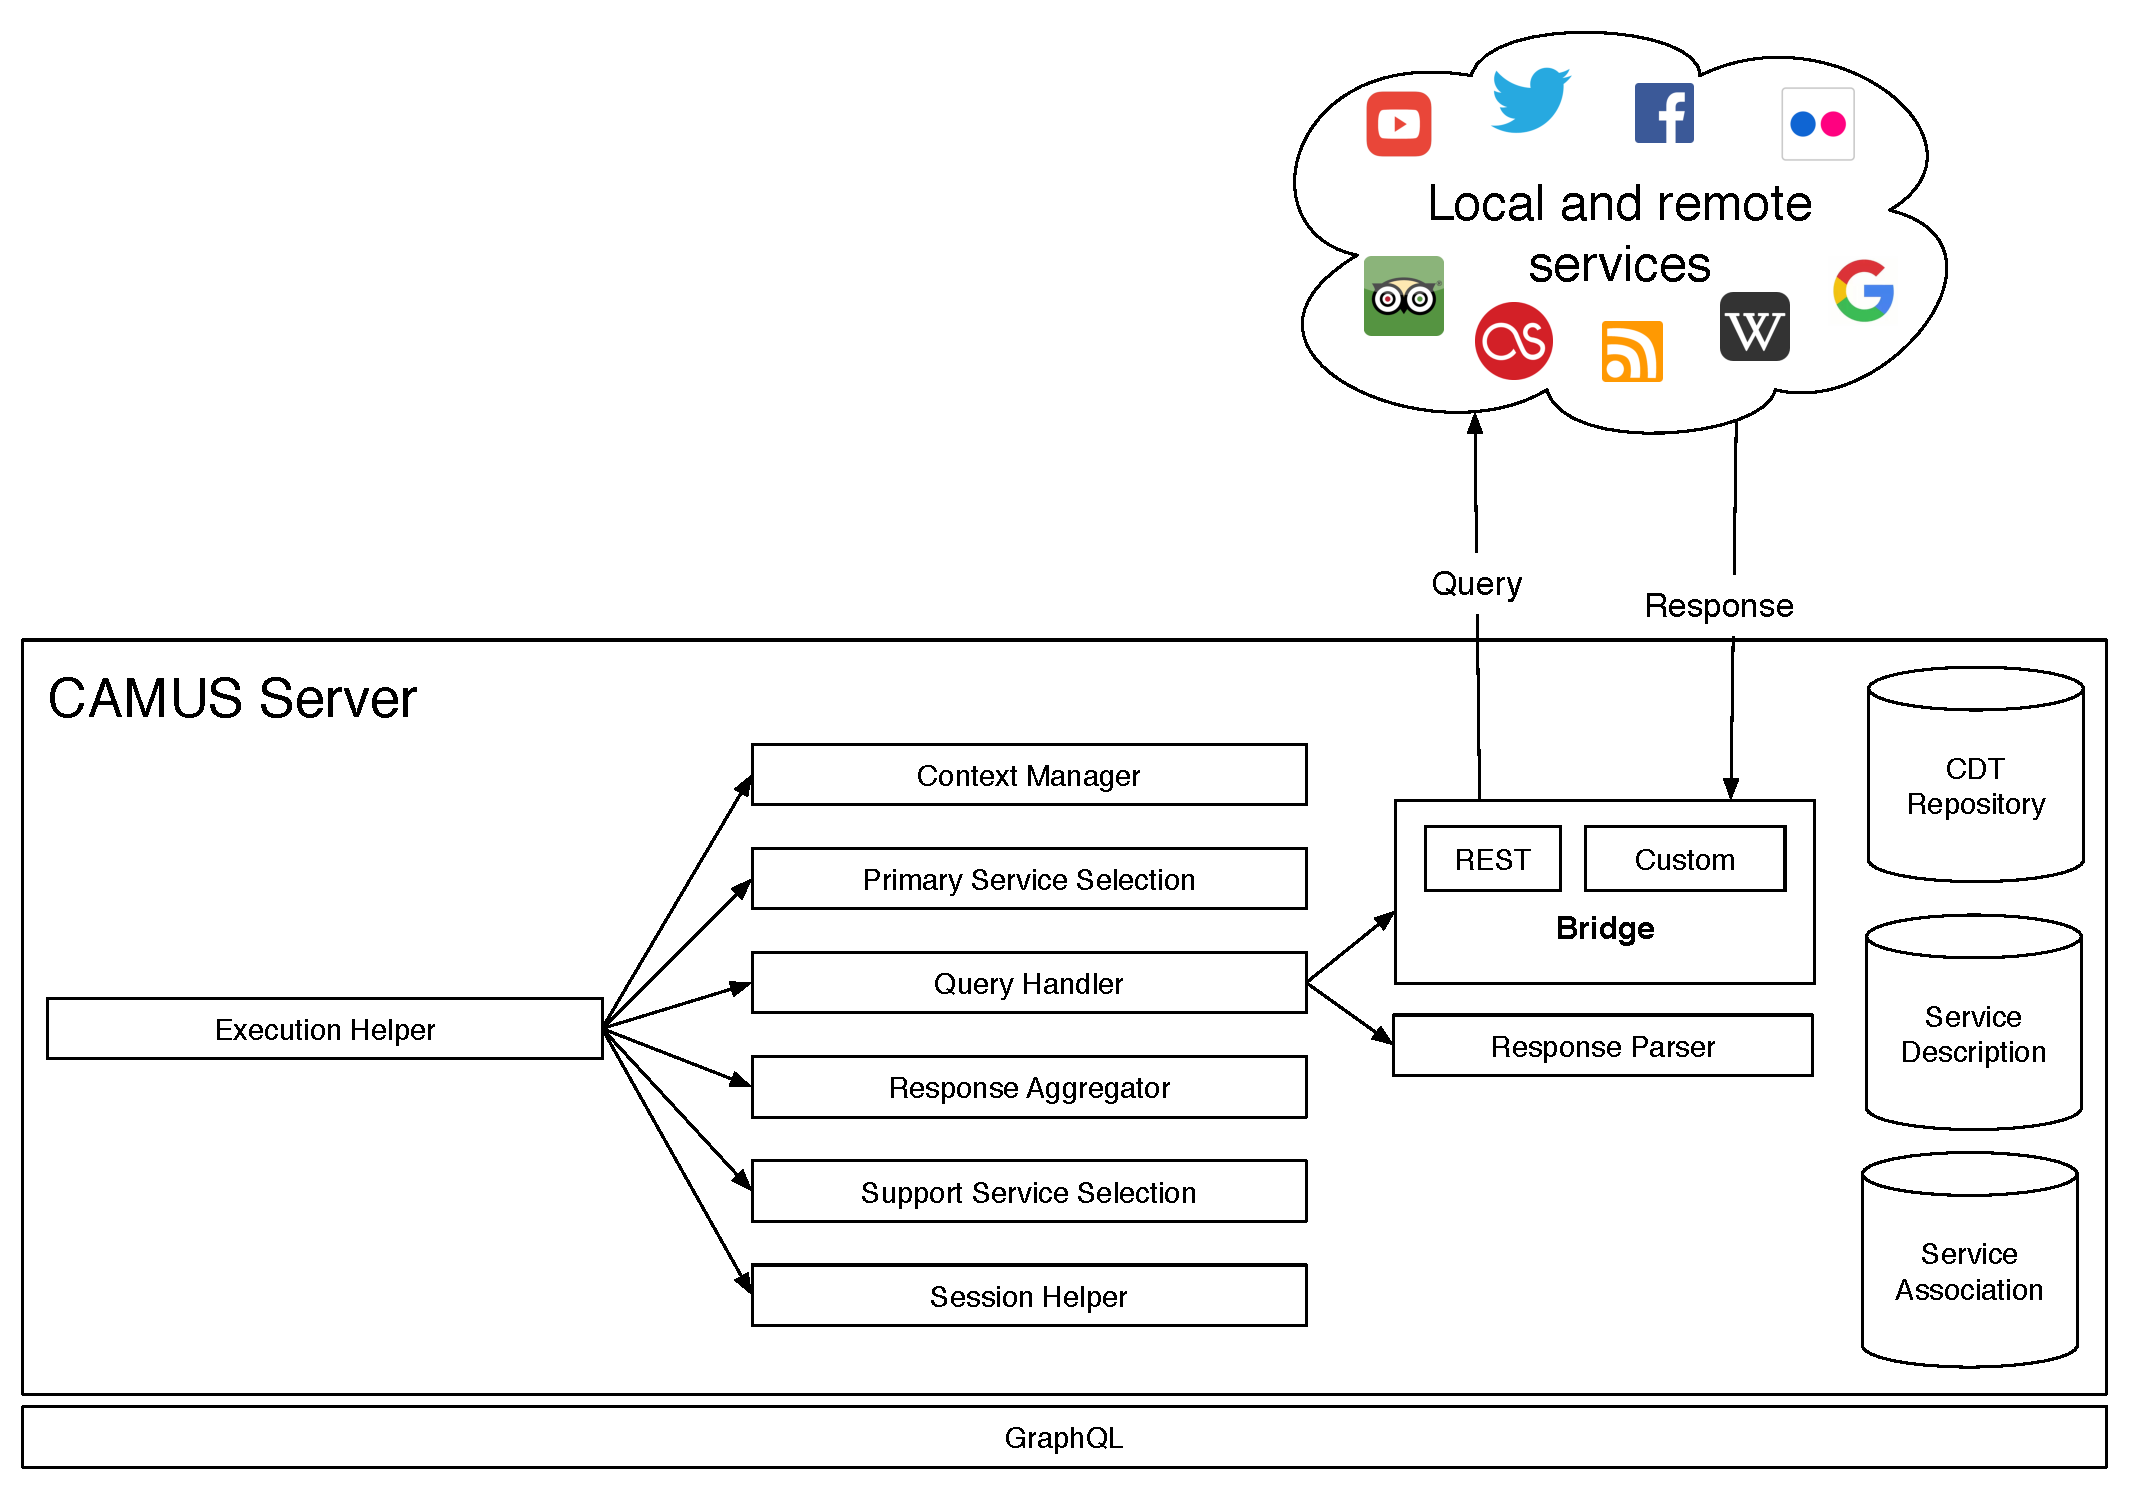
\includegraphics[width=\textwidth]{4-progettazione-alto-livello/Immagini/camus-architecture-backend.pdf}
	\caption{Architettura del backend}\label{fig:architettura-backend}
\end{figure}

L'architettura di CAMUS viene descritta schematicamente in Figura \ref{fig:architettura-backend}. Come si può notare è stata privilegiata la modularità dei vari componenti che formano il sistema, in modo che il compito di ognuno fosse ben circoscritto. Inoltre tutti i componenti mostrati sono \emph{stateless}, cioè non mantengono informazioni sullo stato di una sessione. Questa scelta architetturale permette di poter avviare diverse istanze del \emph{backend} di CAMUS per poter soddisfare le molteplici richieste degli utenti. Questa scelta permette di selezionare quale nodo sia il miglior candidato per gestire una richiesta in coda in base a politiche che non riguardano lo stato della sessione (es.: disponibilità del nodo, basso carico sul sistema, ecc.).

Il componente che coordina tutti gli altri è l'\emph{Execution Helper}. Il suo compito è quello di inizializzare tutti gli altri componenti e organizzare le chiamate secondo il flusso della richiesta (che verrà analizzato nel dettaglio nella Sezione \ref{sec:flusso-richiesta}).

Il \emph{Context Manager} è il componente che si occupa di ricevere il contesto inviato dalla mobile \emph{app} e trasformarlo in una versione \virgolette{decorata}, eseguendo un'unione tra le informazioni ricevute dal \emph{client} e quelle del descrittore completo del CDT. In questo modo viene agevolata l'esecuzione dei componenti successivi, in quanto le informazioni necessarie all'elaborazione sono già state catalogate e definite in modo corretto.

L'attività del \emph{Primary Service Selection} è di andare a recuperare le associazioni tra l'albero di contesto e le operazioni dei servizi primari. \upe inoltre suo compito gestire le associazioni personalizzate, come quella relativa alla ricerca tramite \emph{località}. In seguito assegna un \emph{punteggio} a ogni operazione identificata ed emette in uscita le prime \emph{N} operazioni con valutazione più elevata.

Un compito simile viene svolto dal \emph{Support Service Selection} per le operazioni di supporto. Sebbene lo scopo del componente sia lo stesso, l'algoritmo di selezione è differente: in questo caso viene effettuato un \emph{conteggio} del numero di associazioni trovate e successivamente si verifica che soddisfi il minimo numero di associazioni definito per ogni operazione. Infine, una volta che le operazioni idonee sono state selezionate, vengono composti gli indirizzi, che possono essere sia relativi a \emph{servizi web} oppure degli \emph{intent} verso applicazioni installate sul dispositivo dell'utente. Al \emph{client} sarà richiesto solamente di interrogare il servizio o aprire l'applicazione specificata.

Il \emph{Query Handler} ha il compito di gestire le chiamate verso i servizi primari. Acquisisce l'elenco di operazioni scelte dal \emph{Primary Service Selection} e ne recupera i \emph{descrittori}, contenenti le informazioni per poterli interrogare. Successivamente organizza le chiamate ai servizi attraverso l'uso di \emph{bridge} specifici, scelti in base al \emph{protocollo} di comunicazione adottato dal servizio. Una volta ricevute le risposte, si occupa di interfacciarsi con il \emph{Response Parser} per trasformarle nella rappresentazione interna, che utilizza dei \emph{termini semantici} per associare il rispettivo significato ai vari attributi che compongono la risposta.

Il \emph{Response Aggregator} riceve l'elenco dei risultati dal \emph{Query Handler} e si occupa di andare ad analizzarli per trovare e fondere assieme le entità duplicate e assegna un punteggio a ogni elemento in base alla rilevanza con i dati del contesto (es.: vicinanza del luogo rispetto alla posizione dell'utente, ecc.). Questa attività rende possibile l'ordinamento dei dati in base a criteri di idoneità rispetto alla situazione dell'utente.

Il \emph{Session Helper} si occupa di gestire le richieste verso pagine successive alla prima, in quanto questa attività richiede una fase di preparazione aggiuntiva. Il componente analizza lo stato della richiesta e smista i dati quando sono disponibili altrimenti effettua nuove richieste verso i servizi per acquisire ulteriori informazioni.

Per quanto riguarda l'esposizione dei metodi che possono essere richiamati dal \emph{client} si è deciso di non utilizzare un approccio basato sull'esposizione di \emph{endpoint} \emph{REST} bensì di sperimentare \emph{GraphQL}.

In questa sezione si è voluta dare una visione d'insieme sui compiti che spettano ai vari componenti. Un'analisi più approfondita delle attività di ognuno di essi verrà svolta nella Sezione \ref{sec:componenti-backend}.

\subsection{Mobile app}\label{sec:architettura-applicazione}

In questa sezione è presentata l'architettura dell'applicazione mobile CAMUS, spiegando in modo rapido le diverse tipologie di moduli che la compongono. Si è voluta seguire principalmente un'architettura simile alle applicazioni web per quanto riguarda il controllo della navigazione e della visualizzazione e per quanto riguarda la logica seguire le linee guida di Alt.js. Guardando lo schema presente in Figura \ref{fig:app-architecture} è possibile distinguere diverse tipologie di moduli: le pagine dell'applicazione, gli \emph{helpers} e i componenti che gestiscono lo stato (\emph{Actions} e \emph{Stores}).

\begin{figure}[h]
	\centering
	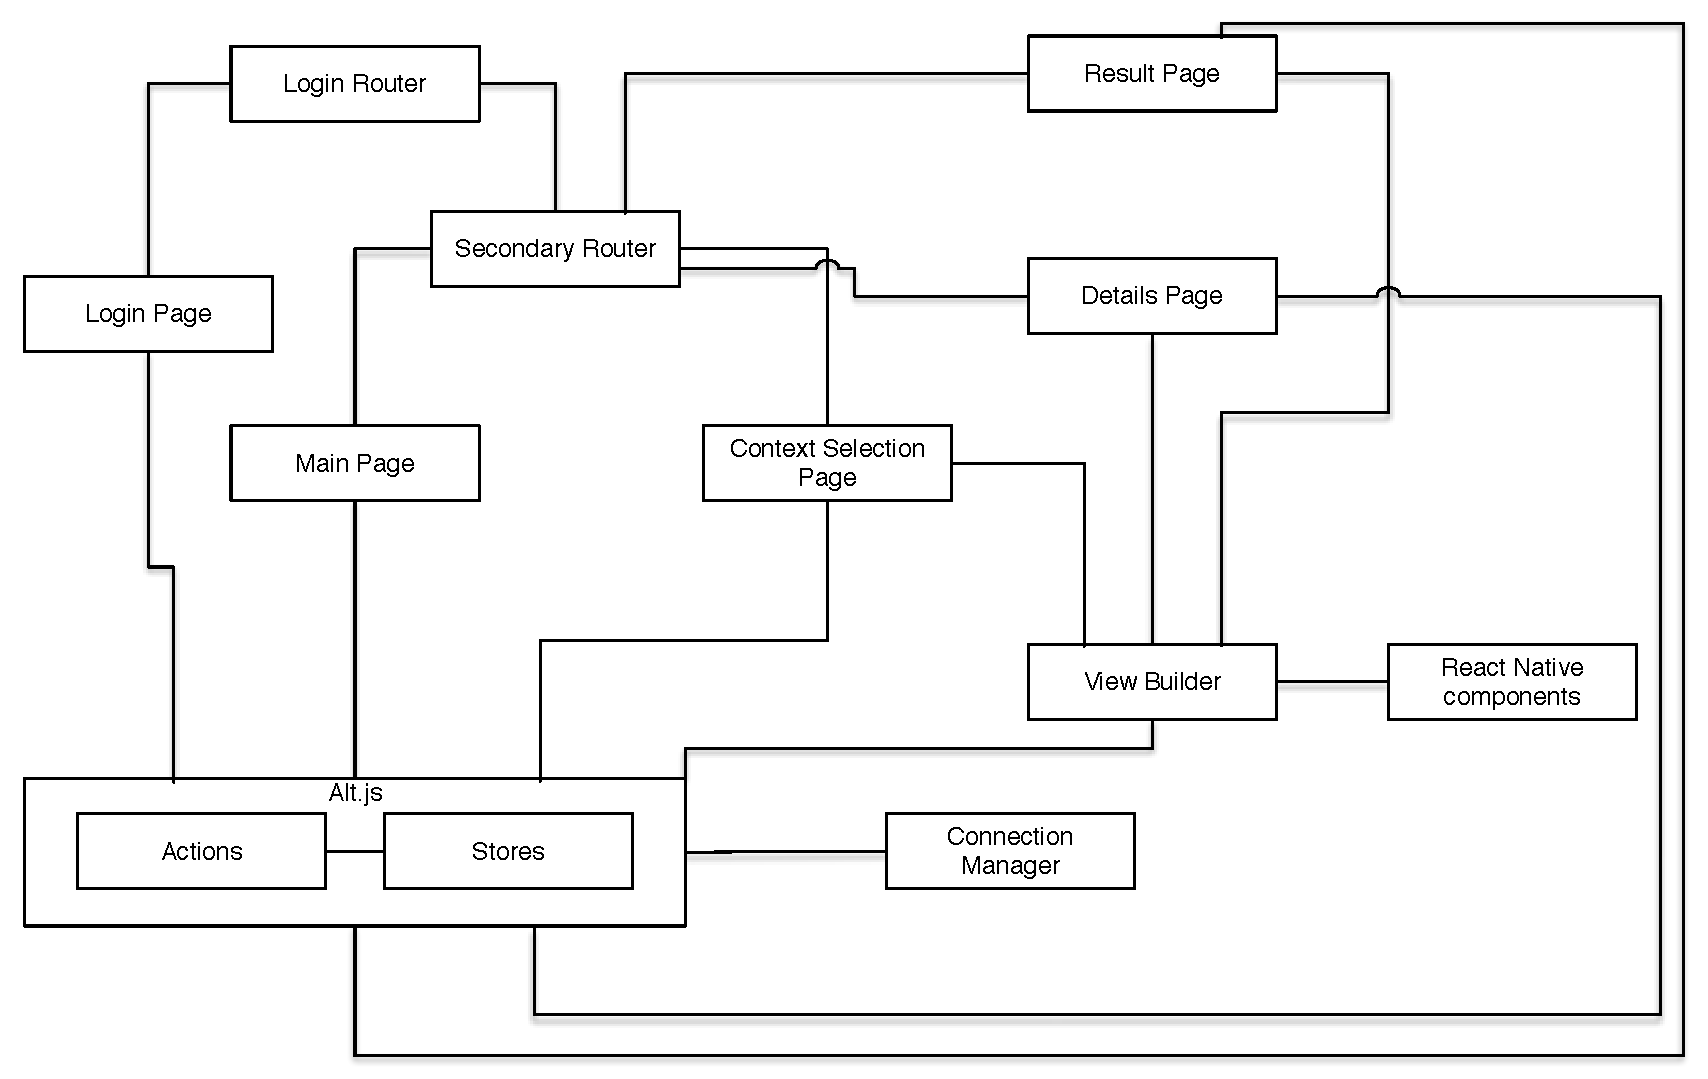
\includegraphics[width=\textwidth]{4-progettazione-alto-livello/Immagini/app_architecture.pdf}
	\caption{Architettura della mobile app}\label{fig:app-architecture}
\end{figure}

\subsubsection{Pagine dell'applicazione}

Essendo un progetto basato su JavaScript per poter controllare le diverse pagine dell'applicazione è necessario utilizzare un \emph{router}. Si è scelto di sfruttare due \emph{router} diversi, uno per gestire il \emph{login} e un altro per la navigazione all'interno dell'applicazione. Il \emph{router} per il \emph{login} controlla solamente se l'utente è loggato e ha lo scopo di non permettere l'accesso alle pagine che necessitano di autenticazione. Come percorsi include \emph{Login Page} e il \emph{secondary router}, che racchiude il controllo della navigazione effettiva una volta che l'utente si è autenticato.

\begin{figure}[H]
	\centering
	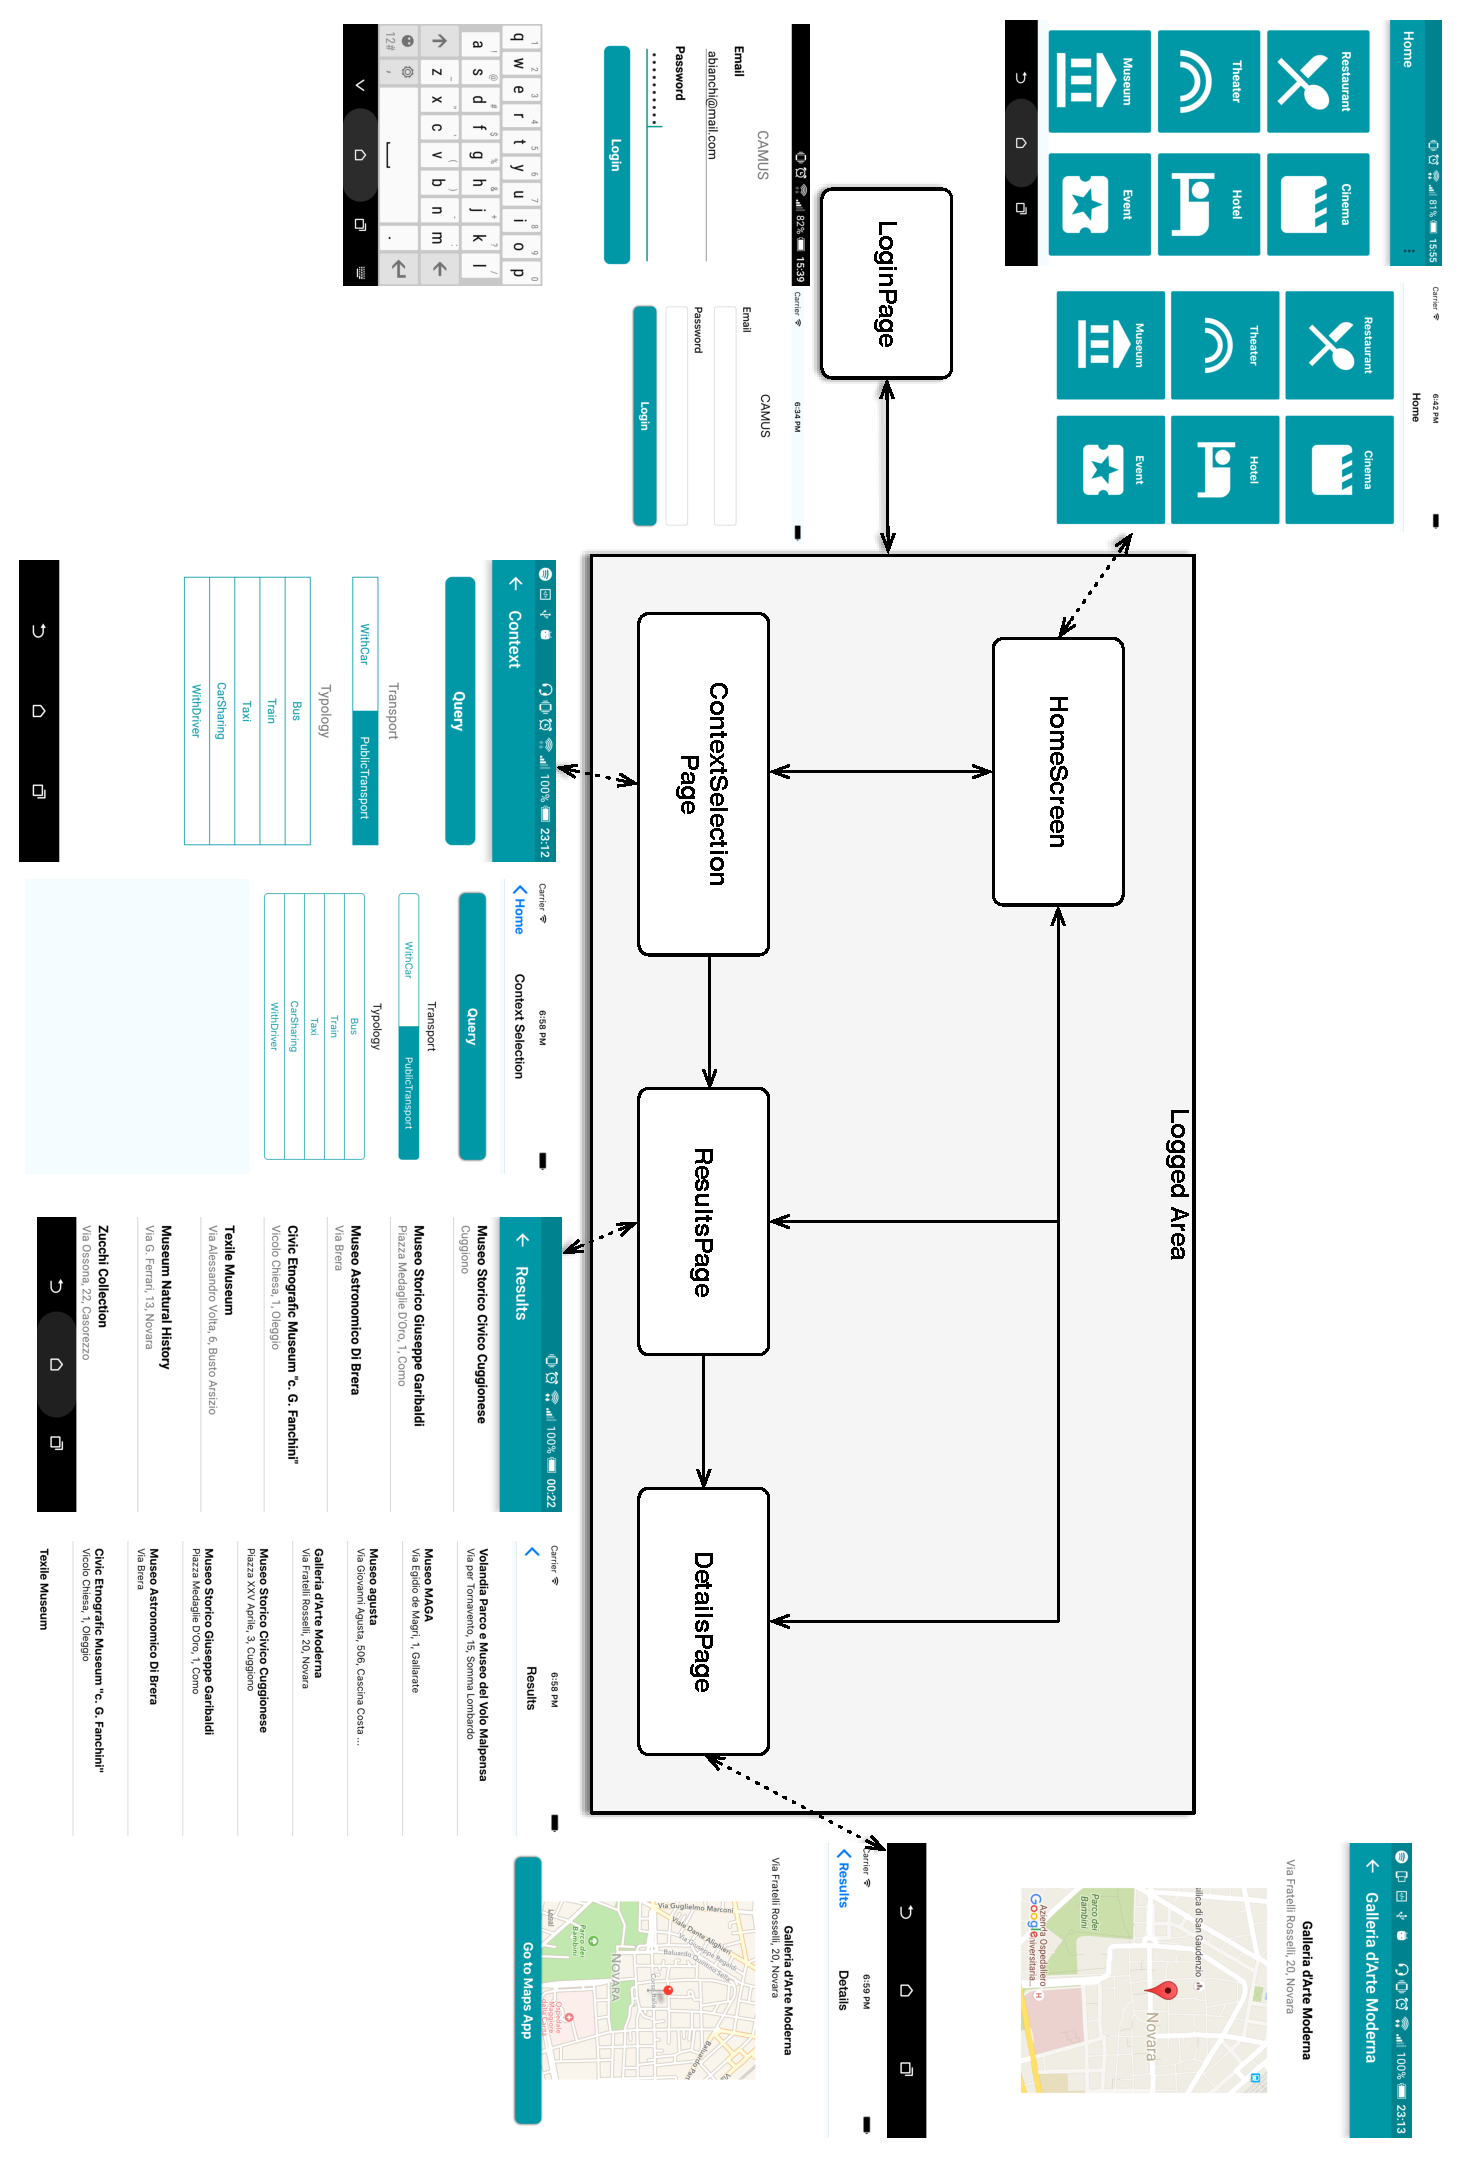
\includegraphics[height=\textwidth, angle=90]{4-progettazione-alto-livello/Immagini/screen_schema.pdf}
	\caption{Schema delle pagine}\label{fig:screen-schema}
\end{figure}
\newpage
Come si può notare nella Figura \ref{fig:screen-schema}, le pagine attraverso cui è possibile navigare sono le seguenti:

\begin{itemize}
	\item \textbf{Login Page}
	\upe la pagina dove l'utente inserisce le proprie credenziali per accedere al sistema CAMUS e ottenere i parametri per il corretto funzionamento dell'applicazione
	\item \textbf{Logged Area}
	Si tratta della parte dell'applicazione alla quale l'utente può accedere nel caso in cui sia autenticato e gestisce le pagine di selezione del contesto e di visualizzazione dati:
	\begin{itemize}
		\item \textbf{Main Page}
		È la pagina principale dell'applicazione e permette all'utente di mostrare tutti gli \emph{Interest Topic} presenti nel suo CDT. La scelta della categoria desiderata permette di accedere alla \emph{Context Selection Page}
		\item \textbf{Context Dimension Page}
		In questa pagina viene chiesto il contesto all'utente mediante un'interfaccia che si adatta a \emph{runtime} man mano che l'utente effettua delle scelte per guidarlo nella definizione del contesto da inviare come richiesta al \emph{server}. Una volta composto il contesto viene costruita la \emph{query} e inviata all'\emph{endpoint} GraphQL del \emph{server} CAMUS. 
		\item \textbf{Results Page}
		Si tratta della pagina che deve mostrare l'intero \emph{dataset} proveniente dal \emph{server} e gestisce la paginazione dei risultati, a seconda della posizione del cursore dell'utente nella \emph{ListView} 
		\item \textbf{Details Page}
		In questa pagina vengono visualizzati i dettagli dell'oggetto selezionato e sono gestiti i collegamenti con le applicazioni esterne, per mezzo della libreria di \emph{Linking} di React Native o tramite moduli personalizzati
	\end{itemize}
\end{itemize}

\subsubsection{Helpers}

Le pagine descritte nella sezione precedente utilizzano alcuni componenti che sono in comune tra tutte le pagine dell'applicazione in quanto aiutano a eseguire funzionalità comuni. Di seguito sono elencati i componenti che svolgono questo compito:

\begin{itemize}
	\item \textbf{Connection Manager}
	In questo componente vengono gestite tutte le connessioni con l'\emph{endpoint} GraphQL. Permette di gestire la fase di \emph{login} e di scambio dati per scaricare il CDT, gli schemi di \emph{mashup} e i dati. Per quanto riguarda i dati sono esposti due metodi distinti, il primo per gestire la prima richiesta di nuovi dati, il secondo per quelle successive, chiedendo una nuova pagina come spiegato nella Sezione \ref{sec:paginazione-app}
	\item \textbf{View Builder}
	Si tratta del componente che costruisce le \emph{view} dinamiche partendo dallo schema di \emph{mashup}, scaricato assieme al CDT appena effettuato il \emph{login}	
	\item \textbf{StyleSheet}
	Si tratta del foglio di stile nel quale sono impostati tutti i parametri predefiniti per la visualizzazione dei componenti dell'applicazione
\end{itemize}

\subsubsection{Actions e Stores\label{sec:action-store}}
Per quanto riguarda la gestione dello stato dell'applicazione si è scelto di seguire in modo piuttosto rigoroso le linee guida fornite da \emph{Alt.js}: le \emph{Action} e le \emph{Store} devono essere collegate tra di loro e riguardare delle funzionalità specifiche.
Per questo motivo sono state create quattro tipologie di coppie \emph{Action-Store} che hanno il compito di gestire il salvataggio dei diversi dati dello stato dell'applicazione: 
\begin{enumerate}
	\item \textbf{User} Ha il compito di gestire tutti i dati anagrafici legati all'utente
	\item \textbf{Data} Memorizza tutto quello che riguarda i dati per l'applicazione, come il CDT e i risultati che provengono dal \emph{server}
	\item \textbf{View} Gestisce gli schemi di \emph{mashup} e il loro aggiornamento all'interno dell'applicazione
	\item \textbf{Context} Ha il compito di memorizzare le scelte in base al contesto fatte dall'utente, permettendo di guidarlo nella definizione della propria situazione
\end{enumerate}

Queste tipologie verranno spiegate nei dettagli nella Sezione \ref{sec:state-management}.

\section{Scenario d'uso}
Viene introdotto un esempio di caso d'uso reale, che vuole il flusso di esecuzione delle attività dell'utente a partire dal \emph{login} fino alla visualizzazione della pagina dei dettagli. Verranno mostrate le attività inizialmente lato \emph{client}, mettendo in evidenza le attività svolte dall’utente, e lato \emph{backend}, descrivendo come viene elaborata la richiesta.
Introduciamo l'utente Andrea, che sarà il nome di fantasia che utilizzeremo in questo esempio. Supponiamo che si deve recare per un weekend a Milano con la sua fidanzata Barbara. Prima di partire ha comunicato a Giovanni, l’esperto CAMUS, del suo progetto di viaggio. Giovanni configura l’applicazione CAMUS personalizzata per Andrea con le informazioni del contesto che gli saranno utili a Milano. Terminato questo lavoro, Giovanni ritiene inoltre che siano utili delle modifiche all'interfaccia grafica dell'applicazione di Andrea.
Qualche giorno più tardi Andrea e Barbara si trovano a Milano in zona Centro e stanno cercando un posto dove poter andare a cena, dato che ormai sono quasi le 20:00. Andrea apre la propria applicazione CAMUS sul suo \textit{smartphone} e inserisce le proprie credenziali di accesso, dato che è la prima volta che la utilizza (Figura \ref{fig:usecase-login}). 

Eseguita l'autenticazione con successo, ad Andrea viene mostrata la schermata principale con la possibilità di scegliere l'\emph{Interest Topic} desiderato tra quelli disponibili (Figura \ref{fig:usecase-home}). La scelta ricade su quello più appropriato: \virgolette{Restaurants}.

\begin{figure}[H]
	\centering
	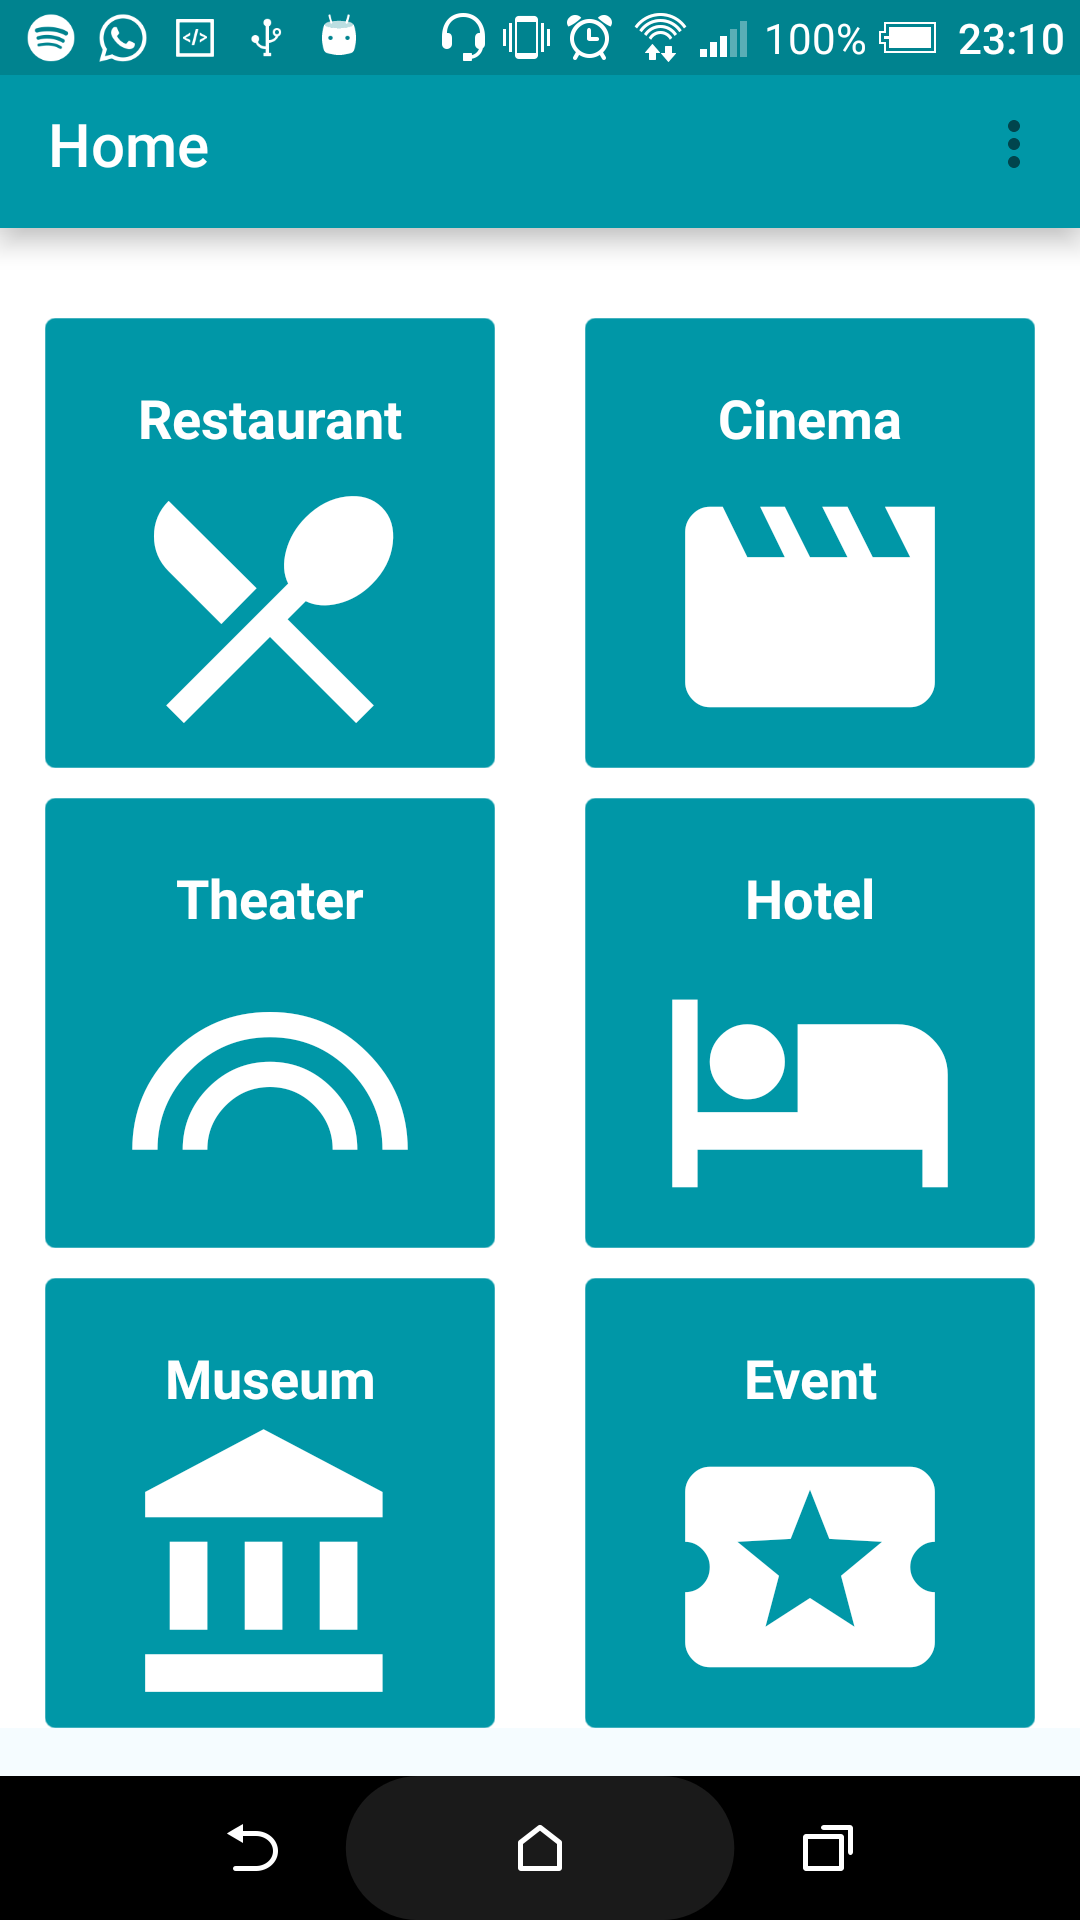
\includegraphics[width=0.35\textwidth]{4-progettazione-alto-livello/Immagini/home_caso_d'uso.png}
	\caption{Schermata principale di Andrea}\label{fig:usecase-home}
\end{figure}

A questo punto è necessario completare il contesto per poter effettuare la richiesta dei ristoranti. Il sistema propone la schermata di selezione del contesto, permettendo nel loro caso di scegliere solamente i mezzi di trasporto, dato che gli altri parametri del profilo di Andrea erano già stati inseriti da Giovanni. Essendo arrivati a Milano utilizzando il treno, viene inserita la possibilità di raggiungere il ristorante con i mezzi pubblici, in particolare con i bus (Figura \ref{fig:usecase-contesto}). 

\begin{figure}[H]
	\centering
	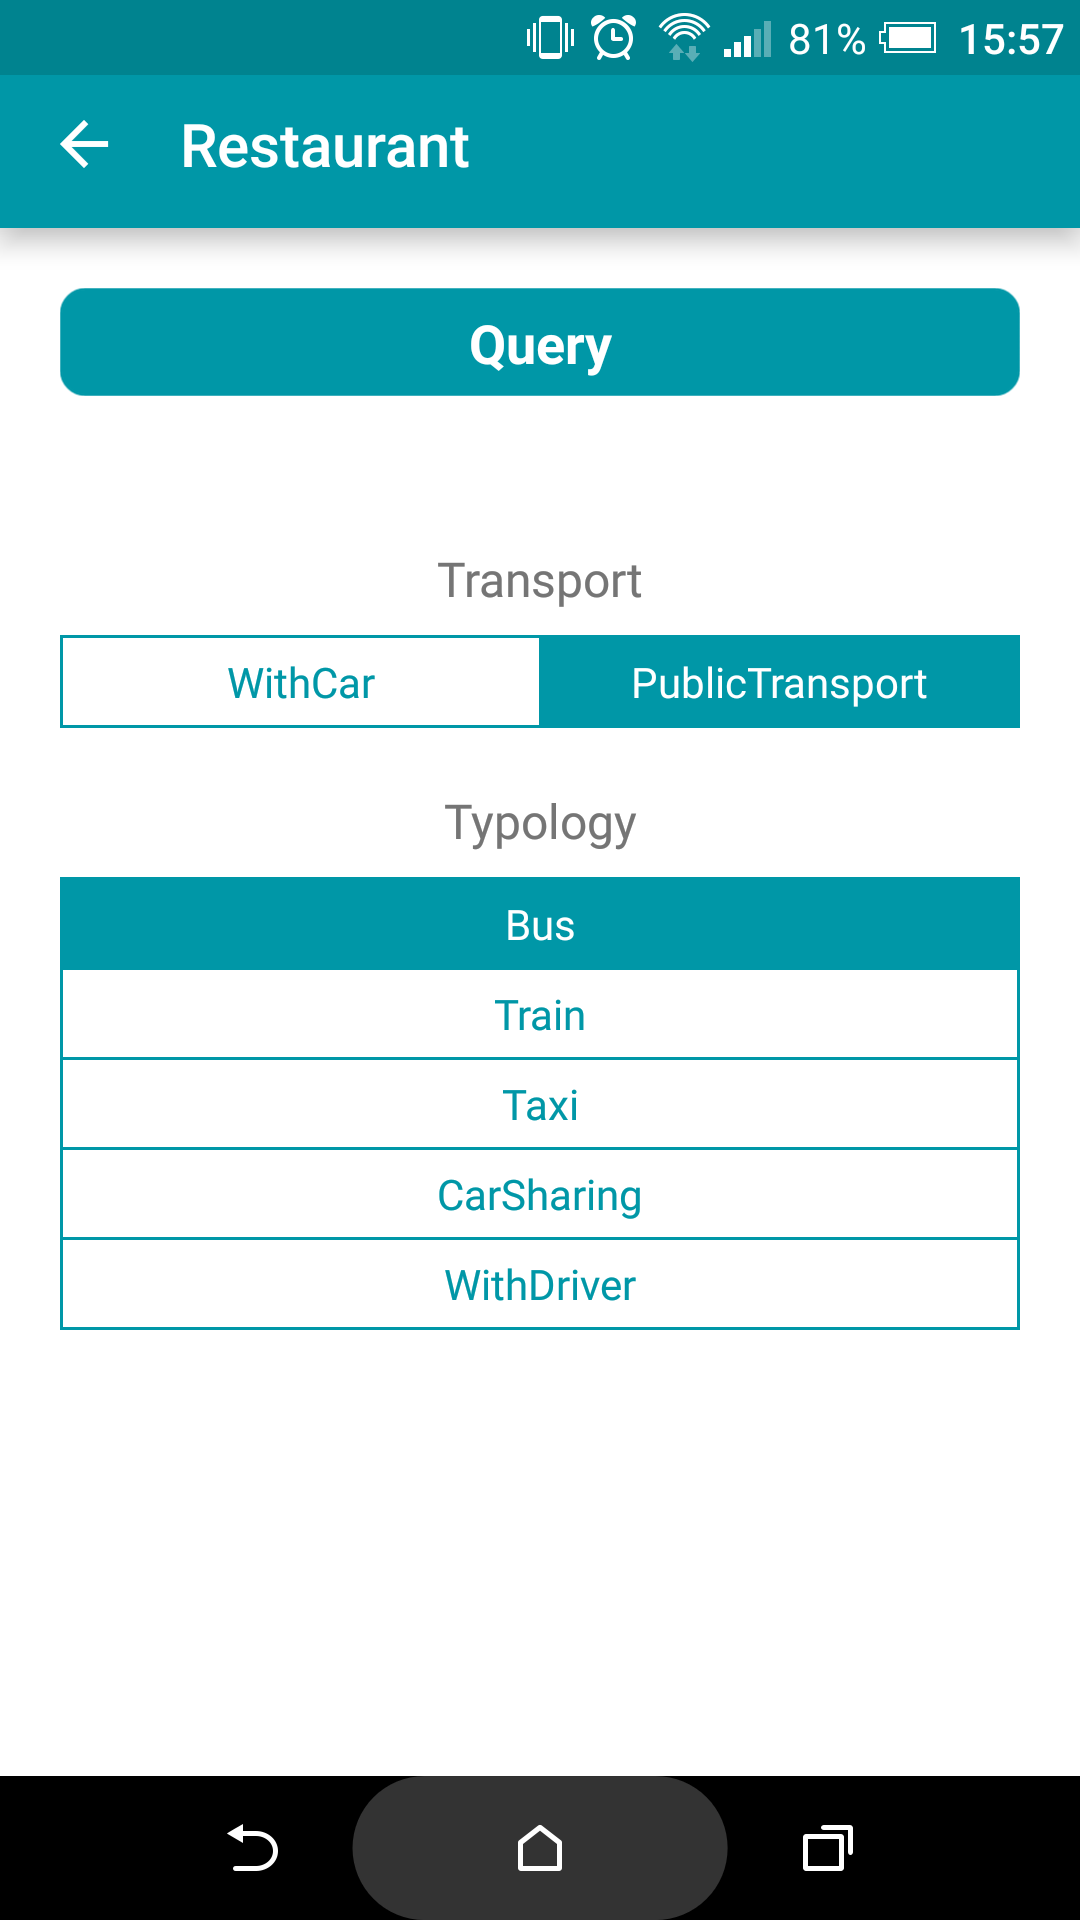
\includegraphics[width=0.35\textwidth]{4-progettazione-alto-livello/Immagini/contesto_caso_d'uso.png}
	\caption{Selezione del contesto}\label{fig:usecase-contesto}
\end{figure}

Selezionando \virgolette{Query} viene costruita la \emph{query}, prendendo i termini dagli schemi di \emph{mashup} e il contesto appena inserito, e inviata al \emph{server}, il quale seleziona i servizi da invocare in base al contesto appena ricevuto, li interroga e costruisce l'insieme di risultati da restituire all'applicazione. Dopo qualche secondo Andrea riceve sul suo \emph{smartphone} la prima pagina dei risultati da lui richiesti, cioè la \textit{view} \emph{ResultsPage} (Figura \ref{fig:usecase-results}).

\begin{figure}[H]
	\centering
	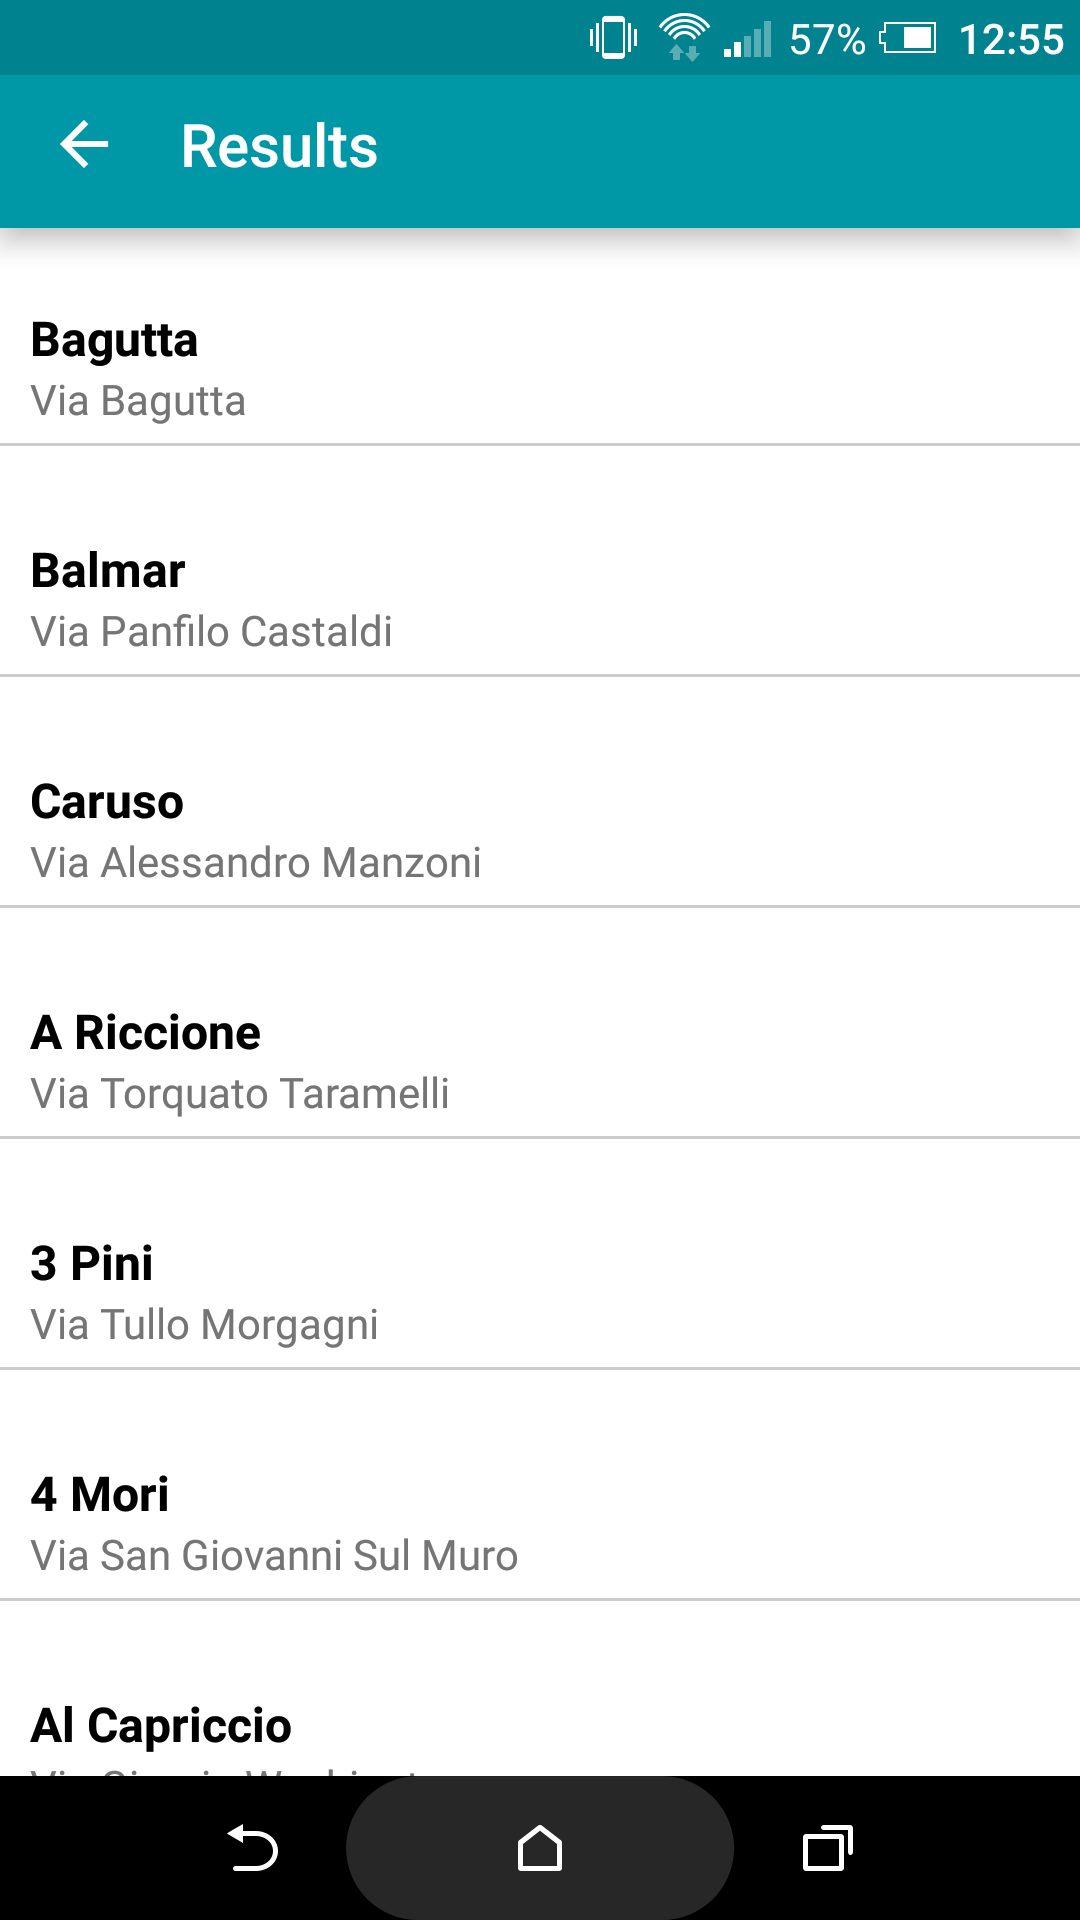
\includegraphics[width=0.35\textwidth]{4-progettazione-alto-livello/Immagini/results_caso_d'uso.png}
	\caption{Risultati ricevuti, mostrati nella \emph{view ResultsPage}}\label{fig:usecase-results}
\end{figure} 

Dopo una rapida consultazione con Barbara, Andrea seleziona il ristorante \virgolette{Caruso} per vedere dei dettagli in più. Quindi, viene create dinamicamente la pagina \emph{DetailsPage} Convinti della scelta e scoprendo che è raggiungibile anche a piedi, decidono di provare a telefonare per prenotare un tavolo per due persone, selezionando il simbolo della cornetta (Figura \ref{fig:usecase-details}). Il ristoratore conferma la prenotazione quindi Andrea e Barbara possono recarsi a cena. %e a passare una piacevole serata.

\begin{figure}[H]
	\centering
	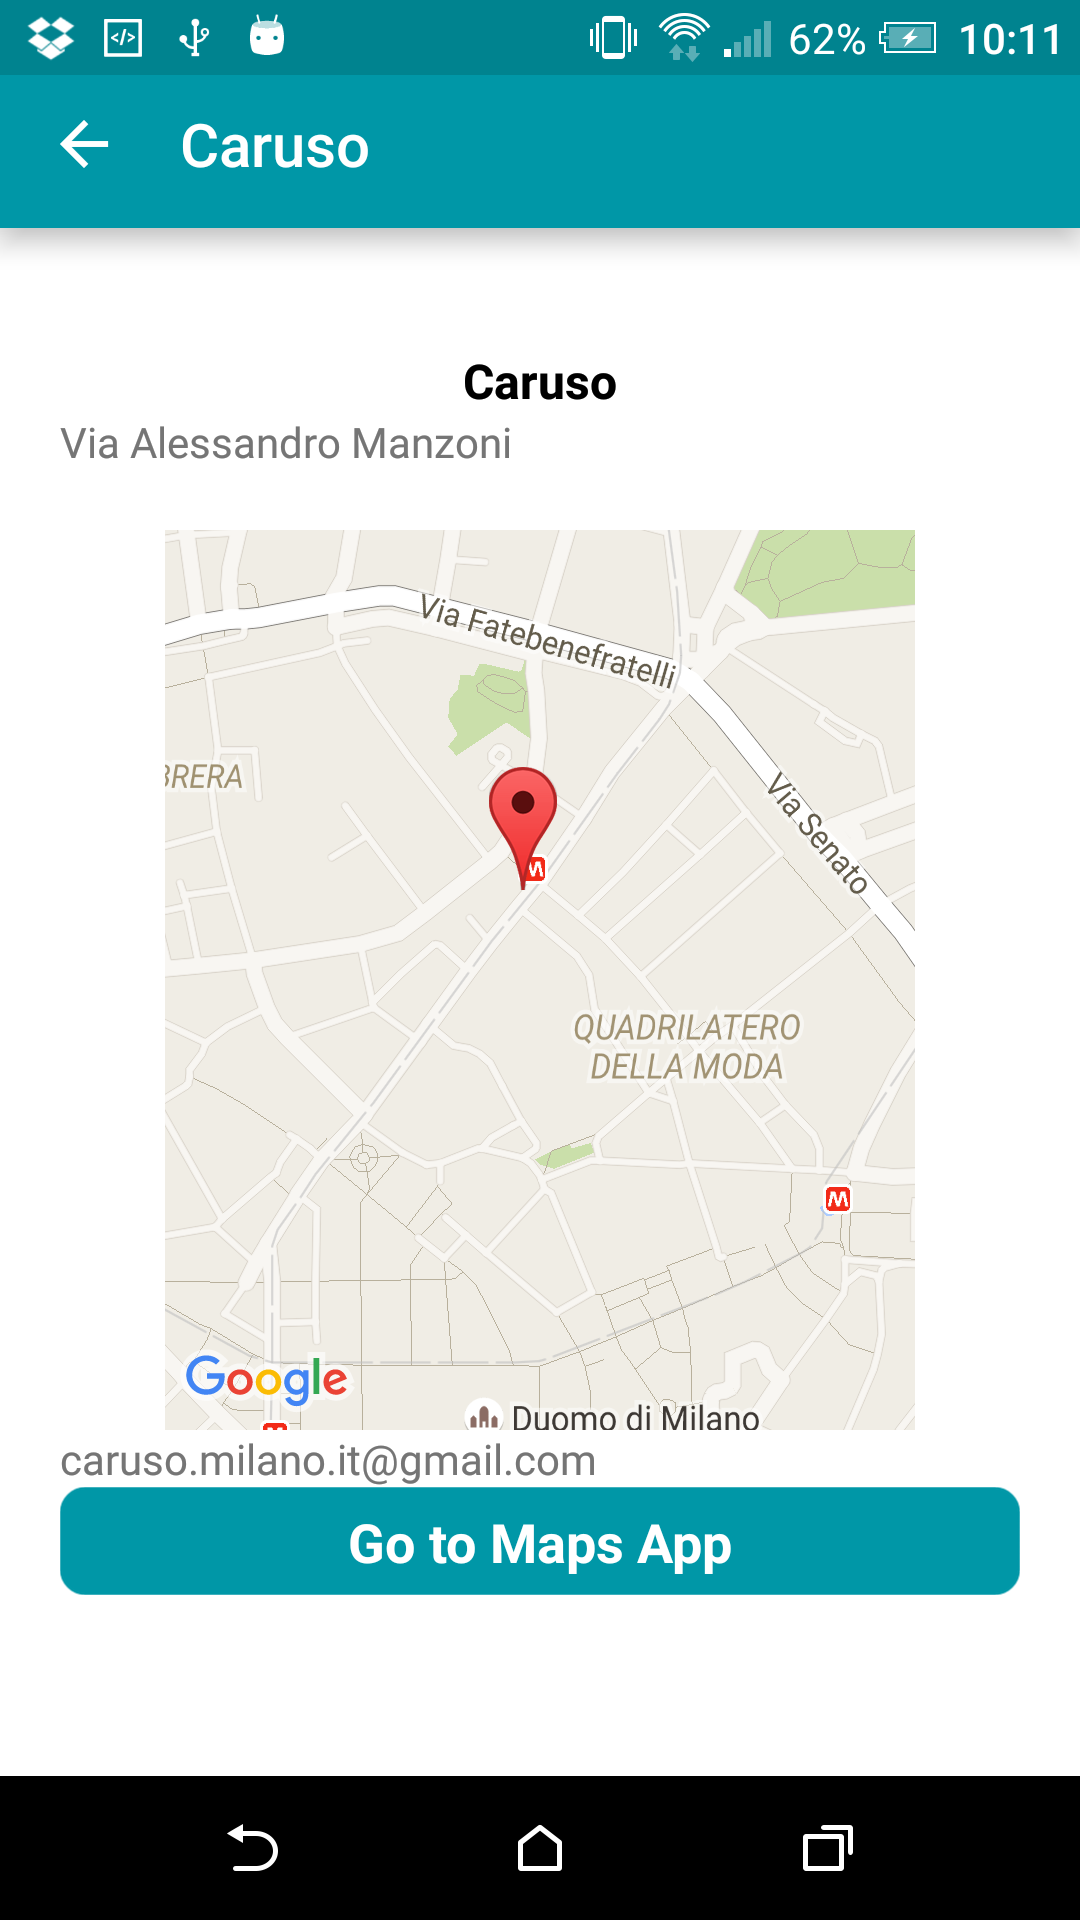
\includegraphics[width=0.35\textwidth]{4-progettazione-alto-livello/Immagini/details_caso_d'uso.png}
	\caption{Dettagli oggetto selezionato (\emph{view DetailsPage})}\label{fig:usecase-details}
\end{figure} 

%In questa sezione viene analizzato il flusso di esecuzione principale del sistema, quello che riguarda le richieste proveniente dalla \emph{mobile app}. Le prime attività che svolge sono il \emph{login} dell'utente, tramite l'\emph{endpoint} \virgolette{login} (Sezione \ref{sec:login-endpoint}), e l'acquisizione dei dati personali dell'utente, tramite l'\emph{endpoint} \virgolette{getPersonalData} (Sezione \ref{sec:get-personal-data-endpoint}).

%L'attività più importante riguarda invece l'\emph{endpoint} \virgolette{executeQuery} (Sezione \ref{sec:execute-query-endpoint}), che è dedicato all'invio delle informazioni trovate in base al contesto dell'utente. In Figura \ref{fig:flusso-nuova-richiesta} vengono mostrati i componenti coinvolti in questa fase e l'ordine col quale sono eseguiti.

\section{Flusso di una richiesta\label{sec:flusso-richiesta}}

Questa sezione vuole mostrare al lettore il flusso di esecuzione delle attività all'interno della piattaforma. Nella sezione precedente si è parlato di un caso d'uso reale mentre ora si vuole entrare nel dettaglio delle attività svolte dal prototipo. Nelle Figure \ref{fig:app-dataflow} e \ref{fig:flusso-nuova-richiesta} vengono mostrati i diagrammi delle attività svolte rispettivamente dalla \emph{mobile app} e dal server, che sono stati separati per mostrare con maggiore chiarezza tutti i passaggi.

%L'attività viene divisa in tre fasi:

%\begin{enumerate}
%	\item \textbf{Creazione CDT decorato}
%	\upe la prima fase che viene eseguita. Una volta ricevuto il contesto dal \emph{client}, questo viene analizzato e trasformato nella versione \emph{decorata}
%	\item \textbf{Acquisizione dati primari}
%	Questa fase avviene dopo la creazione del CDT decorato. Si occupa di selezionare le operazioni attinenti al contesto, interrogare i servizi, integrare le risposte e inviare i dati finali al \emph{client}
%	\item \textbf{Composizione servizi di supporto}
%	Questa fase avviene dopo la creazione del CDT e in parallelo all'acquisizione dei dati primari. A partire dal contesto si occupa di selezionare i servizi di supporto richiesti dal \emph{client} e ne compone le \emph{query}
%\end{enumerate}

%Nelle successive sottosezioni verranno analizzate nel dettaglio ognuna delle precedenti fasi.

\begin{figure}[ht]
	\centering
	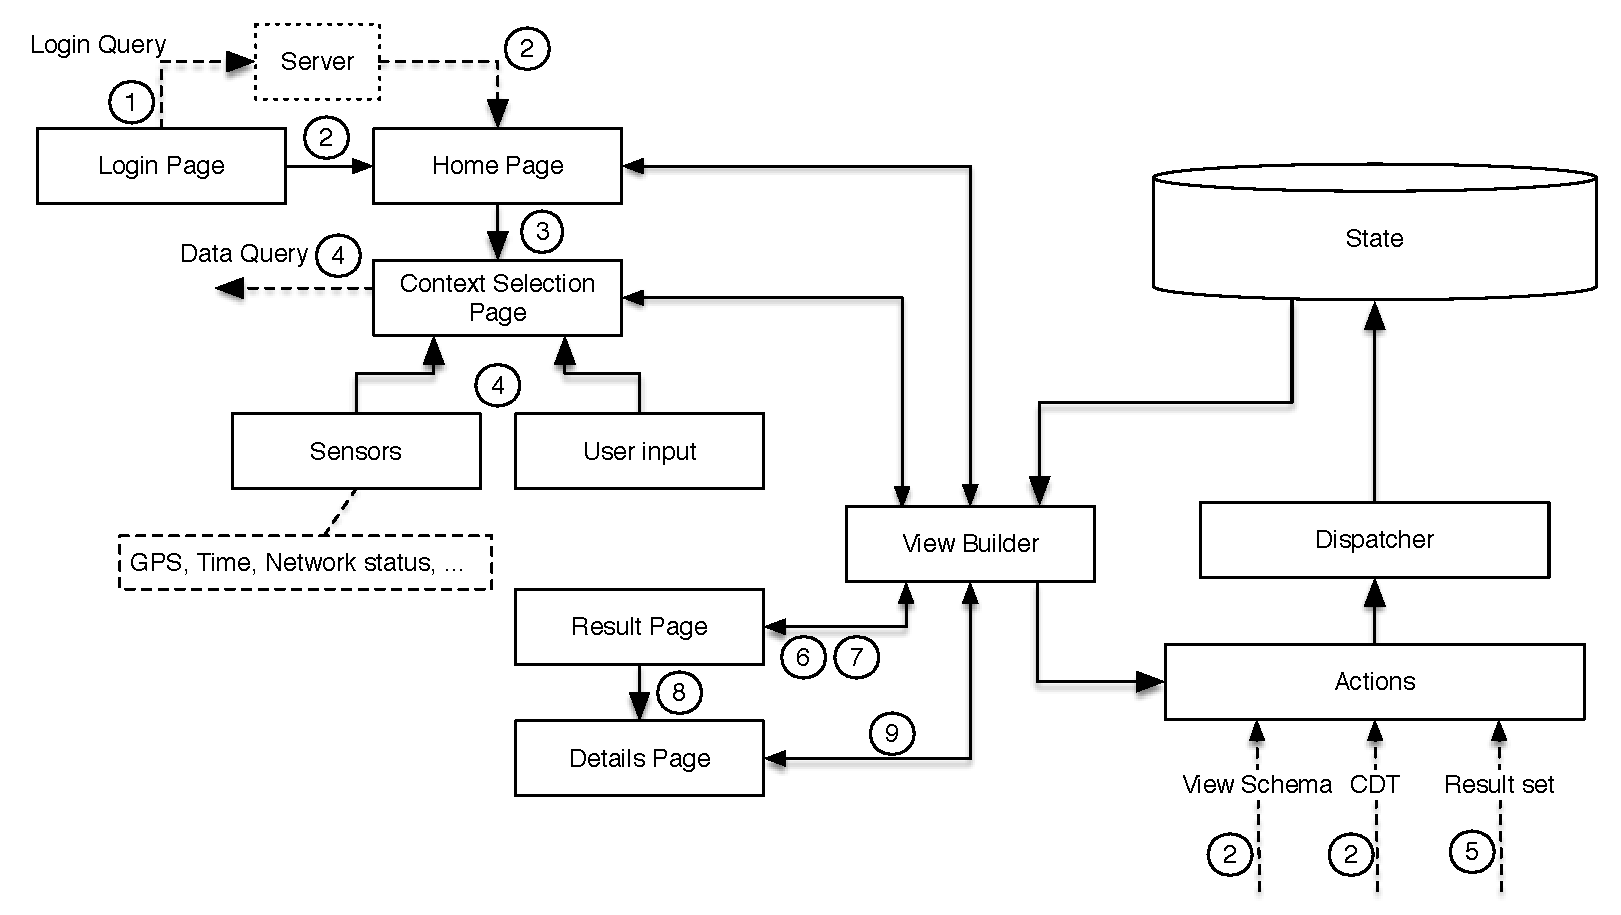
\includegraphics[width=\textwidth]{4-progettazione-alto-livello/Immagini/app_dataflow.pdf}
	\caption{Flusso dei dati dell'app Flux}\label{fig:app-dataflow}
\end{figure}

\begin{figure}[ht]
	\centering
	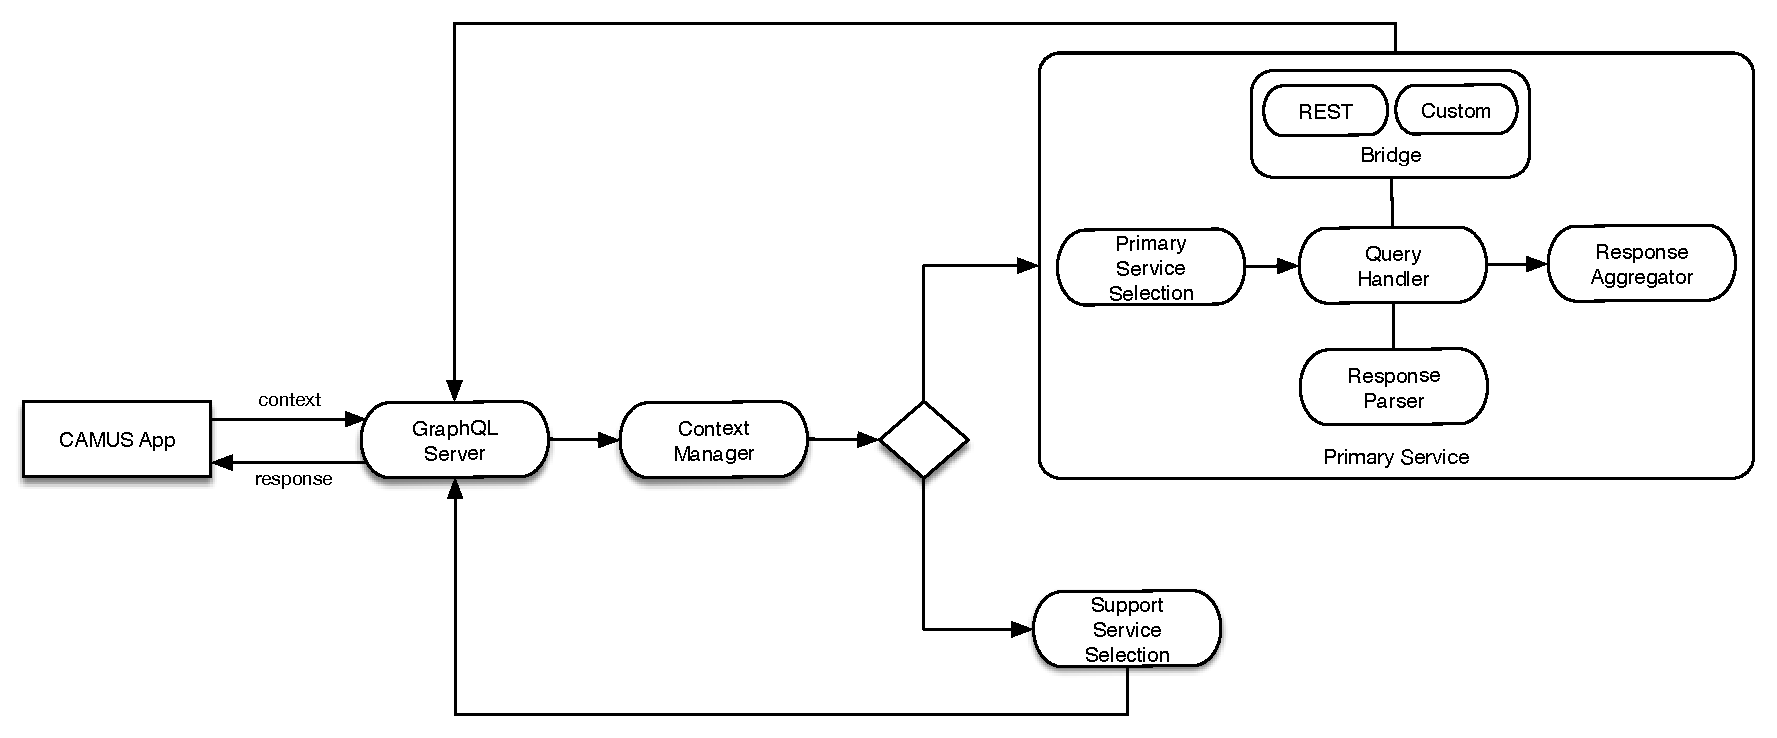
\includegraphics[width=\textwidth]{4-progettazione-alto-livello/Immagini/flusso-richiesta-backend.pdf}
	\caption{Flusso di una nuova richiesta\label{fig:flusso-nuova-richiesta}}
\end{figure}

Per mantenere coerenza con lo scenario d'uso, nelle seguenti sottosezioni si partirà con la fase di autenticazione dell'utente e alla selezione del contesto nella \emph{mobile app}. Verrà in seguito mostrato l'invio del contesto al server e i passaggi necessari per la selezione e l'interrogazione dei servizi. In conclusione, una volta che la \emph{mobile app} riceve i dati, verrà mostrata la modalità di presentazione di queste informazioni e le modalità di interazione.

\subsection*{Login}

La prima schermata che appare nell'applicazione è quella di \emph{login}; qui l'utente inserisce le proprie credenziali e viene effettuata la richiesta GraphQL di \emph{login} come definito nella Sezione \ref{sec:login-endpoint}.
Vengono ricevuti il CDT e i \emph{mashup} personalizzati per l'utente, così che l'applicazione possieda tutto ciò che è necessario per comporre l'interfaccia grafica e mostrare la \emph{view} di selezione dell'\emph{Interest Topic}.

\subsection*{Contesto}

L’utente seleziona l’\emph{Interest Topic} desiderato e viene reindirizzato alla pagina di selezione del contesto dove vengono mostrati i campi che possono essere compilati.
Dopo aver definito i parametri del contesto, l’utente preme il pulsante per effettuare la richiesta al server: l’applicazione recupera i dati inseriti e allo stesso tempo i dati di posizione provenienti dai sensori del dispositivo.
I dati di contesto sono composti assieme ai termini semantici provenienti dagli schemi di \emph{mashup} per costruire la \emph{query} GraphQL. Il \emph{router} dell’applicazione mostra all’utente la pagina dei risultati, la quale durante l’attesa della risposta del server, notifica il caricamento tramite un'animazione grafica. Il server riceve il contesto e ne inizia l'elaborazione.
La prima attività che viene eseguita è la creazione del CDT decorato, della quale si occupa il \emph{Context Manager}. In Figura \ref{fig:flusso-decorated-cdt} viene mostrato il diagramma di flusso delle attività svolte. Riceve in ingresso il \emph{contesto} che è stato composto dall'utente e lo trasforma nella relativa versione \emph{decorata}. Se il contesto è già stato ricevuto in una precedente richiesta, viene recuperata dalla \emph{cache} la versione decorata che è già stata elaborata, altrimenti viene avviato il processo di trasformazione. Al fine di identificare univocamente ogni contesto viene generato un \emph{hash} dell'oggetto ricevuto per poterlo memorizzare e recuperare in \emph{cache}. In questo modo è possibile anche condividere un contesto tra più utenti diversi.

\begin{figure}[ht]
	\centering
	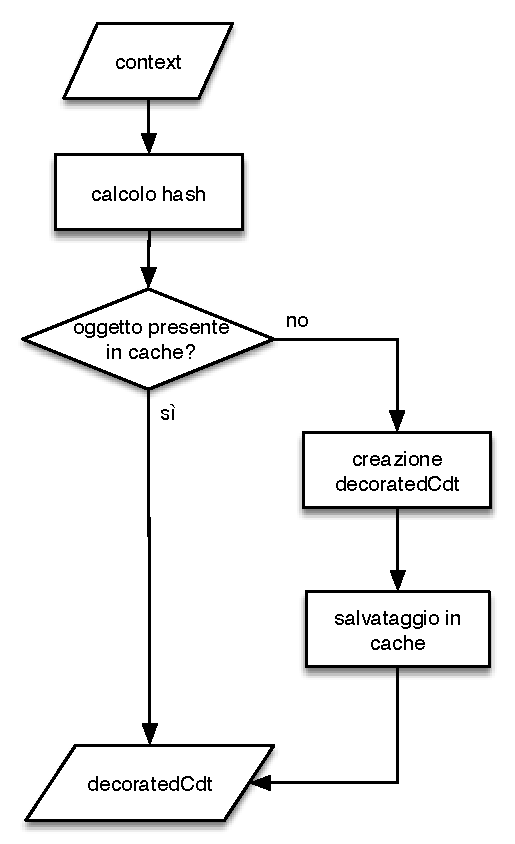
\includegraphics[width=0.43\textwidth]{4-progettazione-alto-livello/Immagini/diagramma_flusso_decoratedCdt.pdf}
	\caption{Flusso di creazione del CDT decorato\label{fig:flusso-decorated-cdt}}
\end{figure}

\begin{figure}[!t]
	\centering
	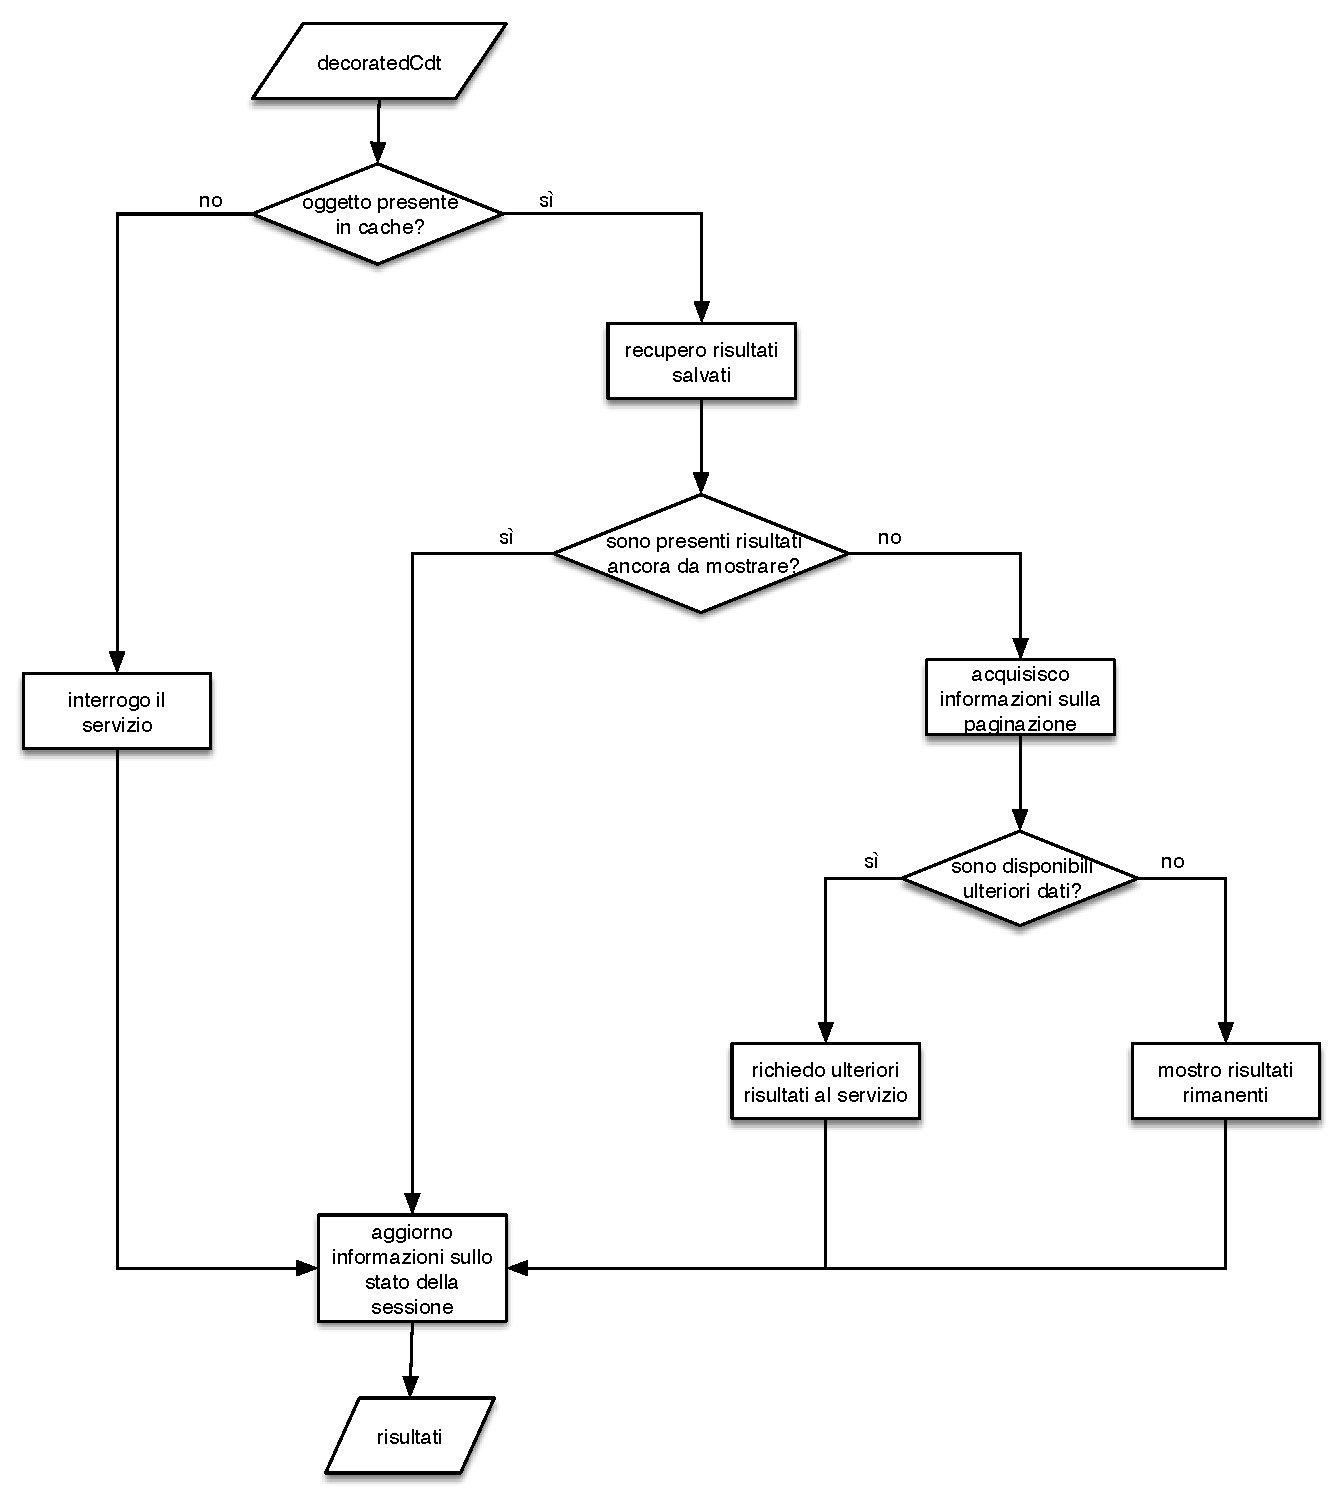
\includegraphics[width=\textwidth]{4-progettazione-alto-livello/Immagini/diagramma_flusso_servizi_primari.pdf}
	\caption{Flusso di richiesta dei risultati primari\label{fig:flusso-servizi-primari}}
\end{figure}

L'operazione successiva è la selezione dei servizi primari. Viene eseguita una volta terminata la creazione del \emph{CDT decorato}. In Figura \ref{fig:flusso-servizi-primari} viene mostrato il diagramma di flusso che mostra come viene gestita una richiesta.

La prima attività che viene svolta riguarda il controllo se la richiesta è già stata gestita in passato. Se si tratta di una nuova richiesta, l'attività viene svolta dai componenti che fanno parte del blocco \virgolette{Primary Service} nella Figura \ref{fig:flusso-nuova-richiesta}. Il primo componente che viene eseguito è il \emph{Primary Service Selection}, che si occupa di selezionare le operazioni che sono più idonee al contesto fornito dall'utente.

\subsection*{Risultati}

Prodotto l'elenco delle operazioni primari, è necessario effettuare le interrogazioni per acquisire i dati. Per svolgere questo compito entra in gioco il \emph{Query Handler}, che ha un duplice compito: il primo, con l'ausilio di uno o più \emph{Bridge}, è l'interrogazione dei servizi prescelti mentre il secondo è l'acquisizione delle relative risposte. Una volta ricevute le risposte provvede a trasformarle nel formato interno, tramite le funzioni messe a disposizione dal \emph{Response Parser}. Tutte le risposte ricevute vengono infine unite a formare un'unica lista e restituite per essere ulteriormente elaborate dal \emph{Response Aggregator}, che effettua un'attività di rimozione dei duplicati. L'elenco dei risultati identificato verrà dunque salvato per un periodo di tempo in \emph{cache} in modo da poter essere riutilizzato per richieste future.
L'altra eventualità si verifica quando la risposta è presente in \emph{cache}. Questo caso ha una gestione un po' più complessa rispetto al precedente perché viene considerata anche la paginazione dei risultati. La prima verifica riguarda la disponibilità di informazioni da restituire al \emph{client}. Se la quantità di dati contenuti in \emph{cache} è sufficiente a evadere la richiesta viene subito restituita la relativa porzione di informazioni. Altrimenti viene effettuata una nuova richiesta verso i servizi che hanno ulteriori dati da mostrare. La regola di ricaricamento dei dati è la stessa descritta nella Sezione \ref{sec:session-helper}. Qualsiasi casistica termina sempre con l'aggiornamento dello stato nella \emph{cache}, in quanto vengono sia salvati l'elenco dei risultati sia il numero di elementi che il \emph{client} ha già richiesto. Il processo termina una volta che tutti i servizi non ha più dati da mostrare. In quel caso il \emph{client} verrà informato del fatto che non sono più disponibili ulteriori pagine.
L'attività di acquisizione dei servizi di supporto comincia una volta creato il \emph{CDT decorato} e opera parallelamente all'acquisizione dei servizi primari. Coinvolge unicamente il componente \emph{Support Service Selection}, che si occupa di selezionare i servizi di supporto o gli \emph{intent} richiesti dal \emph{client}. In ingresso viene fornita la \emph{categoria} dei servizi che si vuole selezionare in base al contesto fornito.
A questo punto il server è pronto per restituire i risultati all'applicazione, che provvede a processarli seguendo le regole definite negli schemi di \emph{mashup} per mostrare i dati.
La prima \emph{view} mostrata contiene l'elenco dei risultati ricevuti, con poche informazioni per permettere all'utente di avere una panoramica sui singoli elementi. Da questa schermata l'utente può selezionare qualsiasi elemento per visualizzarne i dettagli. Viene dunque mostrata una pagina contenente tutte le informazioni recuperate per l'elemento scelto. Inoltre vengono gestiti i servizi di supporto specificati nello schema di \emph{mashup}, in modo che sia possibile l'interazione con applicazioni di terze parti.